\documentclass[11pt]{article}
\usepackage[margin=0.8in,headheight=14pt]{geometry}
\usepackage{amsmath,amssymb}
\usepackage{enumitem,multicol,needspace,fancyhdr,tikz}
\pagestyle{fancy}
\fancyhf{}
\lhead{\small Midterm 1 Study Guide}
\rhead{\small Name: \rule{1.65in}{0.4pt}}
\cfoot{\thepage}
\newcommand{\wsS}{\vspace*{2.0cm}}
\newcommand{\wsM}{\vspace*{3.1cm}}
\newcommand{\wsL}{\vspace*{5.0cm}}
\newlist{probs}{itemize}{1}
\setlist[probs]{leftmargin=2.8em,itemsep=4pt,topsep=3pt,label={}}
\newcounter{problem}
\newcommand{\prob}[1]{\refstepcounter{problem}\item[\textbf{\theproblem.}]}
\newlist{ans}{itemize}{1}
\setlist[ans]{leftmargin=3.0em,itemsep=5pt,topsep=3pt,label={}}
\newcounter{answer}
\newcommand{\ansitem}[1]{\refstepcounter{answer}\item[\textbf{\theanswer.}]}
\newcommand{\choices}[5]{\begin{enumerate}[label=\textbf{(\Alph*)},leftmargin=2.4em,itemsep=1pt,topsep=4pt]\item #1\item #2\item #3\item #4\item #5\end{enumerate}}
\newcommand{\cfuheading}{%
  \Needspace{11.5cm}%
  \par\smallskip
  \noindent\textbf{Section Quizzes}\par
  \vspace{0.2em}
  \noindent\rule{0.55\linewidth}{0.4pt}\par
  \smallskip
}
\newcommand{\topicdivider}[2]{%
  \Needspace{11.5cm}%
  \par\medskip
  \noindent\textbf{Section #1: #2}\par
  \vspace{0.25em}
  \noindent\rule{\linewidth}{0.6pt}\par
  \medskip
}
\begin{document}
\begin{center}
{\Huge\bfseries Midterm 1 Study Guide}\\[0.4em]
{\large Calculus BC \textbullet\ September 2026}\\[0.9em]
\parbox{0.88\linewidth}{\centering Show all work. Use the blank space after each question. A complete answer key and source list begin after the practice set.}
\end{center}
\vspace{0.8em}
\topicdivider{2.1}{Algebraic and One-Sided Limits}
\Needspace{7cm}
\begin{probs}
\prob{1.} Use an algebraic simplification to help find the limit, if it exists.\[\lim_{x\to25}\frac{\sqrt{x}-5}{x-25}.\] \wsM
\end{probs}
\Needspace{7cm}
\begin{probs}
\prob{2.} For $f(x)=\dfrac{x+5}{|x+5|}$ and $a=-5$, find each limit, if it exists:\[\text{(a) }\lim_{x\to a^-}f(x)\qquad\text{(b) }\lim_{x\to a^+}f(x)\qquad\text{(c) }\lim_{x\to a}f(x).\] \wsM
\end{probs}
\Needspace{5.5cm}
\begin{probs}
\prob{3.} If $f(x)=2x^2+1$, then $\displaystyle\lim_{x\to0}\frac{f(x)-f(0)}{x^2}$ is\choices{$0$}{$1$}{$2$}{$4$}{nonexistent} \wsS
\end{probs}
\cfuheading
\Needspace{7cm}
\begin{probs}
\prob{} Find $\displaystyle\lim_{x\to36}\frac{6-\sqrt{x}}{x-36}$. \wsM
\end{probs}
\Needspace{7cm}
\begin{probs}
\prob{} Let
\[
f(x)=\begin{cases}
x^2-2,&-3<x<3,\\
4,&x=3,\\
x+4,&3<x<\infty.
\end{cases}
\]
Find $\displaystyle\lim_{x\to3}f(x)$. \wsM
\end{probs}
\Needspace{10cm}
\begin{probs}
\prob{} The graph of $f$ is shown. Find (a) $\displaystyle\lim_{x\to1^-}f(x)$, (b) $\displaystyle\lim_{x\to1^+}f(x)$, and (c) $\displaystyle\lim_{x\to1}f(x)$.
\begin{center}
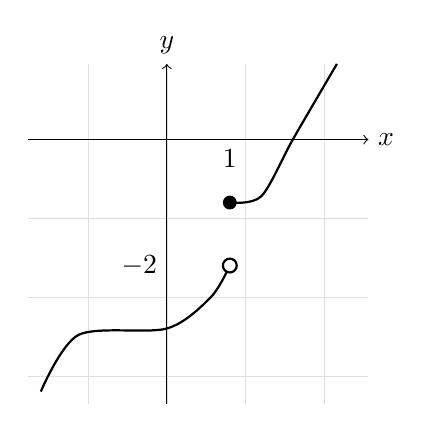
\begin{tikzpicture}[x=0.8cm,y=0.8cm]
  \draw[step=1cm,gray!25,very thin] (-2.2,-4.2) grid (3.2,1.2);
  \draw[->] (-2.2,0)--(3.2,0) node[right] {$x$};
  \draw[->] (0,-4.2)--(0,1.2) node[above] {$y$};
  \draw[thick] plot[smooth] coordinates {(-2,-4) (-1.4,-3.1) (0,-3) (0.7,-2.5) (1,-2)};
  \draw[thick] plot[smooth] coordinates {(1,-1) (1.5,-0.9) (2,0) (2.7,1.2)};
  \draw[fill=white,thick] (1,-2) circle (2.5pt);
  \fill (1,-1) circle (2.5pt);
  \node[left] at (0,-2) {$-2$};
  \node[below] at (1,0) {$1$};
\end{tikzpicture}
\end{center}
\wsM
\end{probs}
\topicdivider{2.2}{The Epsilon-Delta Definition of a Limit}
\Needspace{7cm}
\begin{probs}
\prob{4.} For the given limit $\displaystyle\lim_{x\to4}x^2=16$ and $\varepsilon=0.1$, use the graph of $f$ to find the largest $\delta$ such that if $0<|x-4|<\delta$, then $|f(x)-16|<\varepsilon$. \wsM
\end{probs}
\Needspace{7cm}
\begin{probs}
\prob{5.} Use the $\varepsilon$--$\delta$ definition of a limit to prove that\[\lim_{x\to2}(5x-3)=7.\] \wsM
\end{probs}
\Needspace{5.5cm}
\begin{probs}
\prob{6.} What is $\displaystyle\lim_{h\to0}\frac{8(\frac12+h)^8-8(\frac12)^8}{h}$?\choices{$0$}{$\frac12$}{$1$}{The limit does not exist.}{It cannot be determined from the information given.} \wsS
\end{probs}
\topicdivider{2.3}{Limit Laws and the Squeeze Theorem}
\Needspace{7cm}
\begin{probs}
\prob{7.} Use theorems on limits to find the limit, if it exists.\[\lim_{x\to-3}\frac{x+3}{(1/x)+(1/3)}.\] \wsM
\end{probs}
\Needspace{7cm}
\begin{probs}
\prob{8.} If $0\le f(x)\le c$ for some real number $c$, prove that $\displaystyle\lim_{x\to0}x^2f(x)=0$. \wsM
\end{probs}
\Needspace{5.5cm}
\begin{probs}
\prob{9.} $\displaystyle\lim_{h\to0}\frac{\sin(x+h)-\sin x}{h}$ is\choices{$0$}{$1$}{$\sin x$}{$\cos x$}{nonexistent} \wsS
\end{probs}
\cfuheading
\Needspace{7cm}
\begin{probs}
\prob{} Find $\displaystyle\lim_{x\to2}\left(\frac{x^2}{x-2}-\frac{4}{x-2}\right)$. \wsM
\end{probs}
\Needspace{7cm}
\begin{probs}
\prob{} Find $\displaystyle\lim_{h\to0}\frac{5-\sqrt{25+h}}{h}$. \wsM
\end{probs}
\Needspace{9cm}
\begin{probs}
\prob{} Let $f(x)=\sqrt{7-x}$. Find (a) $\displaystyle\lim_{x\to7^-}f(x)$, (b) $\displaystyle\lim_{x\to7^+}f(x)$, and (c) $\displaystyle\lim_{x\to7}f(x)$. \wsL
\end{probs}
\topicdivider{2.4}{Infinite Limits and Asymptotes}
\Needspace{7cm}
\begin{probs}
\prob{10.} For $f(x)=\dfrac{8}{(2x+5)^3}$ and $a=-\dfrac52$, express each limit as $\infty$, $-\infty$, or DNE (Does Not Exist):\[\text{(a) }\lim_{x\to a^-}f(x)\qquad\text{(b) }\lim_{x\to a^+}f(x)\qquad\text{(c) }\lim_{x\to a}f(x).\] \wsM
\end{probs}
\Needspace{7cm}
\begin{probs}
\prob{11.} Find the vertical and horizontal asymptotes for the graph of $f$.\[f(x)=\frac{x^2-5x}{x^2-25}.\] \wsM
\end{probs}
\Needspace{5.5cm}
\begin{probs}
\prob{12.} If $k$ is a positive integer, then $\displaystyle\lim_{x\to+\infty}\frac{x^k}{e^x}$ is\choices{$0$}{$1$}{$e$}{$k!$}{nonexistent} \wsS
\end{probs}
\cfuheading
\Needspace{7cm}
\begin{probs}
\prob{} Evaluate $\displaystyle\lim_{x\to\infty}\frac{-x^4+5x}{3x^3-4}$.\choices{$0$}{$-\frac13$}{$-\infty$}{$\infty$}{$\frac53$} \wsM
\end{probs}
\Needspace{7cm}
\begin{probs}
\prob{} Find $\displaystyle\lim_{x\to-\infty}\frac{5x-3}{\sqrt{x^2+2}}$. \wsM
\end{probs}
\Needspace{8cm}
\begin{probs}
\prob{} Find the horizontal asymptote and all vertical asymptotes of
\[
f(x)=\frac{x^2-2x}{25-x^2}.
\]
\wsM
\end{probs}
\topicdivider{2.5}{Continuity and the Intermediate Value Theorem}
\Needspace{7cm}
\begin{probs}
\prob{13.} Classify the discontinuities of $f$ as removable, jump, or infinite.\[f(x)=\begin{cases}-x^2,&x<1,\\2,&x=1,\\x-2,&x>1.\end{cases}\] \wsM
\end{probs}
\Needspace{7cm}
\begin{probs}
\prob{14.} If $f(x)=x^3-5x^2+7x-9$, use the intermediate value theorem to prove that there is a real number $a$ such that $f(a)=100$. \wsM
\end{probs}
\Needspace{7cm}
\begin{probs}
\prob{15.} Let $f$ be defined by \[f(x)=\begin{cases}\sin x,&x<0,\\x^2,&0\le x<1,\\2-x,&1\le x<2,\\x-3,&x\ge2.\end{cases}\] For what values of $x$ is $f$ NOT continuous?\choices{$0$ only}{$1$ only}{$2$ only}{$0$ and $2$ only}{$0$, $1$, and $2$} \wsM
\end{probs}
\topicdivider{3.1}{Derivatives from the Limit Definition}
\Needspace{7cm}
\begin{probs}
\prob{16.} Let $f(x)=3-2x^2$. (a) Use the limit definition to find the slope of the tangent line to the graph of $f$ at $P(a,f(a))$. (b) Find an equation of the tangent line at $P(2,f(2))$. \wsM
\end{probs}
\Needspace{10cm}
\begin{probs}
\prob{17.} A projectile is fired directly upward from the ground with an initial velocity of $112$ ft/sec. Its distance above the ground after $t$ seconds is $112t-16t^2$ feet. (a) Find the velocity of the projectile at $t=2$, $t=3$, and $t=4$. (b) When does the projectile strike the ground? (c) Find the velocity at the instant it strikes the ground. \wsL
\end{probs}
\Needspace{7cm}
\begin{probs}
\prob{18.} For what nonnegative value of $b$ is the line $y=-\frac13x+b$ normal to the curve $y=x^3$?\choices{$0$}{$1$}{$\frac43$}{$\frac{10}{3}$}{$\frac{10\sqrt3}{3}$} \wsM
\end{probs}
\cfuheading
\Needspace{9cm}
\begin{probs}
\prob{} Given $y=x^2+3$: (a) find the average rate of change of $y$ with respect to $x$ on $[2,2.1]$; (b) find the instantaneous rate of change at the left endpoint. \wsL
\end{probs}
\Needspace{9cm}
\begin{probs}
\prob{} A sandbag is dropped from a hot-air balloon hovering $600$ feet above the ground. Ignoring air resistance, its height after $t$ seconds is $s(t)=-16t^2+600$. Find its velocity (a) at time $t$ and (b) at $t=2$ seconds. \wsL
\end{probs}
\Needspace{7cm}
\begin{probs}
\prob{} Use the limit definition of slope to find the slope of $f(x)=\sqrt{x}$ at $P(9,3)$.\choices{$1$}{$\frac16$}{$9$}{$\frac19$}{$6$} \wsM
\end{probs}
\topicdivider{3.2}{Differentiability and Tangent Lines}
\Needspace{10cm}
\begin{probs}
\prob{19.} Let $f(x)=x^3-4x$ and $P(2,0)$. (a) Use the definition of the derivative to find $f'(x)$. (b) Find the domain of $f'$. (c) Find an equation of the tangent line to the graph of $f$ at $P$. (d) Find the points on the graph at which the tangent line is horizontal. \wsL
\end{probs}
\Needspace{7cm}
\begin{probs}
\prob{20.} Is $f(x)=\sqrt[3]{x}$ differentiable on the given interval? Explain. (a) $[-1,1]$; (b) $[-2,-1]$. \wsM
\end{probs}
\Needspace{5.5cm}
\begin{probs}
\prob{21.} If $f$ is a function such that $\displaystyle\lim_{x\to2}\frac{f(x)-f(2)}{x-2}=0$, which statement must be true?\choices{The limit of $f(x)$ as $x$ approaches $2$ does not exist.}{$f$ is not defined at $x=2$.}{$f'(2)=0$.}{$f$ is continuous at $x=0$.}{$f(2)=0$.} \wsS
\end{probs}
\cfuheading
\Needspace{7cm}
\begin{probs}
\prob{} If $y=-3x+10$, find $\dfrac{d^3y}{dx^3}$. \wsM
\end{probs}
\Needspace{7cm}
\begin{probs}
\prob{} Evaluate $\displaystyle\lim_{h\to0}\frac{(x+h)^4-x^4}{h}$.\choices{$x^4$}{$(x+h)^4$}{$4x^3$}{$(4x^3)'$}{nonexistent} \wsM
\end{probs}
\Needspace{8cm}
\begin{probs}
\prob{} Let
\[
f(x)=\begin{cases}
3x,&x\le0,\\
x^3,&x>0.
\end{cases}
\]
Find the domain of $f'$. \wsM
\end{probs}
\topicdivider{3.3}{Product, Quotient, and Higher Derivatives}
\Needspace{7cm}
\begin{probs}
\prob{22.} Find the derivative of $G(v)=\dfrac{v^3-1}{v^3+1}$. \wsM
\end{probs}
\Needspace{7cm}
\begin{probs}
\prob{23.} Solve the equation $\dfrac{d^2y}{dx^2}=0$ for $y=6x^4+24x^3-540x^2+7$. \wsM
\end{probs}
\Needspace{7cm}
\begin{probs}
\prob{24.} If $u$, $v$, and $w$ are nonzero differentiable functions, then the derivative of $\dfrac{uv}{w}$ is\choices{$\dfrac{uv'+u'v}{w'}$}{$\dfrac{u'v'w-uvw'}{w^2}$}{$\dfrac{uvw'-u'vw-uv'w}{w^2}$}{$\dfrac{u'vw+uv'w+uvw'}{w^2}$}{$\dfrac{uv'w+u'vw-uvw'}{w^2}$} \wsM
\end{probs}
\cfuheading
\Needspace{7cm}
\begin{probs}
\prob{} Given $f(x)=\dfrac{3x-2}{5x+1}$, find $f'(2)$. Give an exact fraction. \wsM
\end{probs}
\Needspace{8cm}
\begin{probs}
\prob{} Find the derivative of $h(x)=(x^2-4)(x^4+2)$.\choices{$(2x)(4x^3)+(4x^3)(2x)$}{$(x^2-4)(4x^3)-(x^4+2)(2x)$}{$(2x)(4x^3)$}{$(x^2-4)(4x^3)+(x^4+2)(2x)$}{$(x^2-4)(x^4+2)$} \wsM
\end{probs}
\Needspace{8cm}
\begin{probs}
\prob{} If $f(3)=2$, $f'(3)=8$, $g(3)=-3$, and $g'(3)=5$, find (a) $\left(\dfrac1f\right)'(3)$ and (b) $(fg)'(3)$. \wsM
\end{probs}
\Needspace{8cm}
\begin{probs}
\prob{} Find the point $P$ on $y=x^2$ such that the tangent line at $P$ has $x$-intercept $1$. Give an exact answer. \wsM
\end{probs}
\topicdivider{3.4}{Trigonometric Derivatives}
\Needspace{7cm}
\begin{probs}
\prob{25.} Find the derivative of $h(z)=\dfrac{1-\cos z}{1+\cos z}$. \wsM
\end{probs}
\Needspace{7cm}
\begin{probs}
\prob{26.} Find equations of the tangent line and the normal line to the graph of $f(x)=\csc x+\cot x$ at the point $\bigl(\pi/4,f(\pi/4)\bigr)$. \wsM
\end{probs}
\Needspace{7cm}
\begin{probs}
\prob{27.} If $f(x)=\dfrac{x}{\tan x}$, then $f'(\frac\pi4)=$\choices{$2$}{$\frac12$}{$1+\frac\pi2$}{$\frac\pi2-1$}{$1-\frac\pi2$} \wsM
\end{probs}
\cfuheading
\Needspace{7cm}
\begin{probs}
\prob{} If $h(z)=\dfrac{1-\sin z}{1+\cos z}$, find $h'(0)$. \wsM
\end{probs}
\Needspace{7cm}
\begin{probs}
\prob{} Evaluate $\displaystyle\lim_{x\to0}\frac{\sin(2x)}{x}$. \wsM
\end{probs}
\Needspace{7cm}
\begin{probs}
\prob{} If $r(\theta)=\cot\theta+\csc\theta$, find $r'(\pi/6)$. \wsM
\end{probs}
\topicdivider{3.5}{Linear Approximation and Differentials}
\Needspace{10cm}
\begin{probs}
\prob{28.} Let $y=1/x^2$, $a=3$, and $\Delta x=0.3$. (a) Find general formulas for $\Delta y$ and $dy$. (b) If, for the given values of $a$ and $\Delta x$, $x$ changes from $a$ to $a+\Delta x$, find the values of $\Delta y$ and $dy$. \wsL
\end{probs}
\Needspace{10cm}
\begin{probs}
\prob{29.} Constriction of arterioles is a cause of high blood pressure. It has been verified experimentally that, as blood flows through an arteriole of fixed length, the pressure difference between the two ends of the arteriole is inversely proportional to the fourth power of the radius. If the radius of an arteriole decreases by $10\%$, use differentials to find the percentage change in the pressure difference. \wsL
\end{probs}
\Needspace{7cm}
\begin{probs}
\prob{30.} Let $f(x)=x^2-2x+3$. The tangent line to the graph of $f$ at $x=2$ is used to approximate $f(x)$. Which is the greatest value of $x$ for which the error is less than $0.5$?\choices{$2.4$}{$2.5$}{$2.6$}{$2.7$}{$2.8$} \wsM
\end{probs}
\topicdivider{3.6}{The Chain Rule}
\Needspace{7cm}
\begin{probs}
\prob{31.} Find the derivative of $f(x)=\sin\sqrt{x}+\sqrt{\sin x}$. \wsM
\end{probs}
\Needspace{7cm}
\begin{probs}
\prob{32.} Let $p$, $q$, and $r$ be functions such that $p(z)=q(r(z))$. If $r(3)=3$, $q(3)=-2$, $r'(3)=4$, and $q'(3)=6$, find $p(3)$ and $p'(3)$. \wsM
\end{probs}
\Needspace{7cm}
\begin{probs}
\prob{33.} Let $f$ and $g$ be differentiable, with $f(1)=2$, $f'(1)=3$, $f'(2)=-4$, $g(1)=2$, $g'(1)=-3$, and $g'(2)=5$. If $h(x)=f(g(x))$, then $h'(1)=$\choices{$-9$}{$-4$}{$0$}{$12$}{$15$} \wsM
\end{probs}
\cfuheading
\Needspace{8cm}
\begin{probs}
\prob{} Let $m(x)=\tan^2\!\left(\sqrt{x^2-5}\right)$. Find $m'(3)$.\choices{$\tan(2)\sec^2(2)$}{$3\tan(2)\sec^2(2)$}{$4\tan(2)\sec(2)$}{$\frac12\sec^2(6)$}{$\frac14\tan(2)\sec^2(2)$} \wsM
\end{probs}
\Needspace{8cm}
\begin{probs}
\prob{} Use the tangent line to $f(x)=x^2(3-x)$ at $x=1$ to approximate $f(1.1)$. \wsM
\end{probs}
\Needspace{9cm}
\begin{probs}
\prob{} A particle moves along $y=x^3-2$ such that $\dfrac{dx}{dt}=xy$. Find $\dfrac{dy}{dt}$ at $(x,y)=(2,6)$. \wsL
\end{probs}
\topicdivider{3.7}{Implicit Differentiation}
\Needspace{7cm}
\begin{probs}
\prob{34.} Assuming that the equation $x=\sin(xy)$ determines a differentiable function $f$ such that $y=f(x)$, find $y'$. \wsM
\end{probs}
\Needspace{7cm}
\begin{probs}
\prob{35.} Assuming that the equation $3x^2+4y^2=4$ determines a function $f$ such that $y=f(x)$, find $y''$, if it exists. \wsM
\end{probs}
\Needspace{7cm}
\begin{probs}
\prob{36.} The slope of the line tangent to the curve $y^2+(xy+1)^3=0$ at $(2,-1)$ is\choices{$-\frac32$}{$-\frac34$}{$0$}{$\frac34$}{$\frac32$} \wsM
\end{probs}
\cfuheading
\Needspace{7cm}
\begin{probs}
\prob{} Given $x^2-2y^2=18$, find $y'$ at $(6,3)$. \wsM
\end{probs}
\Needspace{7cm}
\begin{probs}
\prob{} Given $xy=\sin y$, find $y'$ at $(0,\pi)$.\choices{$0$}{$1$}{$-1$}{$-\pi$}{$\pi$} \wsM
\end{probs}
\Needspace{9cm}
\begin{probs}
\prob{} The curve $x^2+y^2+\sqrt2xy=1$ has horizontal tangent lines at two points. Find both points. \wsL
\end{probs}
\topicdivider{3.8}{Related Rates}
\Needspace{10cm}
\begin{probs}
\prob{37.} A metal rod has the shape of a right circular cylinder. As it is being heated, its length is increasing at a rate of $0.005$ cm/min and its diameter is increasing at $0.002$ cm/min. At what rate is the volume changing when the rod has length $40$ centimeters and diameter $3$ centimeters? \wsL
\end{probs}
\Needspace{10cm}
\begin{probs}
\prob{38.} A ladder $20$ feet long leans against a vertical building. If the bottom of the ladder slides away from the building horizontally at a rate of $2$ ft/sec, at what rate is the angle between the ladder and the ground changing when the top of the ladder is $12$ feet above the ground? \wsL
\end{probs}
\Needspace{7cm}
\begin{probs}
\prob{39.} A person $2$ meters tall walks directly away from a streetlight $8$ meters above the ground. The person's shadow is lengthening at $\frac49$ meter per second. At what rate, in meters per second, is the person walking?\choices{$\frac4{27}$}{$\frac49$}{$\frac34$}{$\frac43$}{$\frac{16}{9}$} \wsM
\end{probs}
\cfuheading
\Needspace{11cm}
\begin{probs}
\prob{} Tony, who is $6$ ft tall, walks away from an $18$ ft lamppost at $3$ ft/sec. At the moment Tony's head is $24$ ft from the top of the lamppost, find (a) the rate at which the length of Tony's shadow is increasing, (b) the rate at which the tip of the shadow is moving, and (c) the rate at which the acute angle formed by the ground and the line from the shadow's tip to Tony's head is changing. \wsL
\end{probs}
\Needspace{9cm}
\begin{probs}
\prob{} A square has side lengths increasing at $2$ cm/sec. When each side is $6$ cm, find (a) the rate at which the diagonal is changing and (b) the rate at which the area is changing. \wsL
\end{probs}
\topicdivider{3.9}{Chapter 3 Derivative Review}
\Needspace{10cm}
\begin{probs}
\prob{40.} Suppose $f$ and $g$ are functions such that $f(2)=-1$, $f'(2)=4$, $f''(2)=-2$, $g(2)=-3$, $g'(2)=2$, and $g''(2)=1$. Find the value of each of the following at $x=2$: (a) $(2f-3g)'$; (b) $(2f-3g)''$; (c) $(fg)'$; (d) $(fg)''$; (e) $\left(\dfrac fg\right)'$; (f) $\left(\dfrac fg\right)''$. \wsL
\end{probs}
\Needspace{7cm}
\begin{probs}
\prob{41.} Let $f(x)=\begin{cases}(2x-1)^3,&x\ge2,\\5x^2+34x-61,&x<2.\end{cases}$ Determine if $f$ is differentiable at $2$. \wsM
\end{probs}
\Needspace{7cm}
\begin{probs}
\prob{42.} If $f$ and $g$ are twice differentiable and $h(x)=f(g(x))$, then $h''(x)=$\choices{$f''(g(x))[g'(x)]^2+f'(g(x))g''(x)$}{$f''(g(x))g'(x)+f'(g(x))g''(x)$}{$f''(g(x))[g'(x)]^2$}{$f''(g(x))g''(x)$}{$f''(g(x))$} \wsM
\end{probs}
\topicdivider{4.1}{Extrema and Critical Numbers}
\Needspace{10cm}
\begin{probs}
\prob{43.} Find the extrema of $f$ on the given interval. \[f(x)=3x^2-10x+7,\qquad[-1,3].\] \wsL
\end{probs}
\Needspace{7cm}
\begin{probs}
\prob{44.} Find the critical numbers of $k(r)=r^5-2r^3+r-12$. \wsM
\end{probs}
\Needspace{7cm}
\begin{probs}
\prob{45.} If $f(x)=\frac13x^3-4x^2+12x-5$ on $0\le x\le9$, then the absolute maximum value of $f$ occurs when $x$ is\choices{$0$}{$2$}{$4$}{$6$}{$9$} \wsM
\end{probs}
\cfuheading
\Needspace{11cm}
\begin{probs}
\prob{} The graph of $f$ is shown below.
\begin{center}
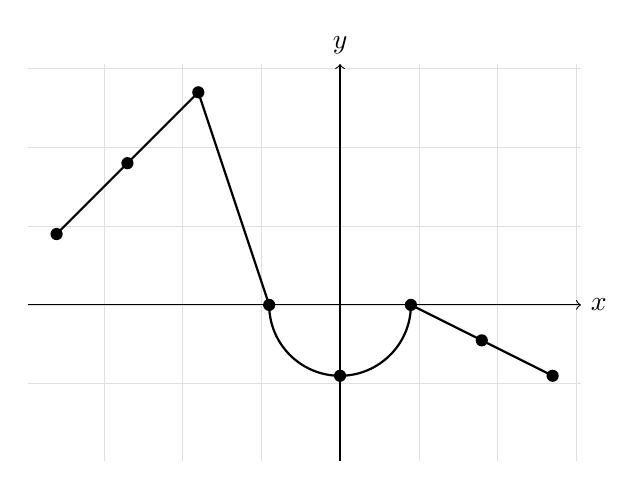
\begin{tikzpicture}[x=0.9cm,y=0.9cm]
  \draw[step=1cm,gray!25,very thin] (-4.4,-2.2) grid (3.4,3.4);
  \draw[->] (-4.4,0)--(3.4,0) node[right] {$x$};
  \draw[->] (0,-2.2)--(0,3.4) node[above] {$y$};
  \draw[thick] (-4,1)--(-2,3)--(-1,0);
  \draw[thick] (-1,0) arc[start angle=180,end angle=360,radius=1];
  \draw[thick] (1,0)--(3,-1);
  \foreach \p in {(-4,1),(-3,2),(-2,3),(-1,0),(0,-1),(1,0),(2,-0.5),(3,-1)} \fill \p circle (2.2pt);
\end{tikzpicture}
\end{center}
Find (a) the maximum value of $f$, (b) the number of critical numbers of $f$ on $(-4,3)$, and (c) the $x$-values where $f$ has a local maximum. \wsM
\end{probs}
\Needspace{8cm}
\begin{probs}
\prob{} Find the absolute maximum value of $y=x^3-4x^2-5$ on $[-2,5]$.\choices{$5$}{$0$}{$-5$}{$20$}{$25$} \wsM
\end{probs}
\Needspace{8cm}
\begin{probs}
\prob{} State the interval on which $y=x^2$ is increasing and the interval on which $y=x^3$ is increasing. \wsM
\end{probs}
\Needspace{8cm}
\begin{probs}
\prob{} Select all critical numbers of $y=\dfrac{x^2+2x-8}{x-4}$ from the list $0,2,4,6,8,10$. \wsM
\end{probs}
\topicdivider{4.2}{Rolle's Theorem and the Mean Value Theorem}
\Needspace{10cm}
\begin{probs}
\prob{46.} Show that $f$ satisfies the hypotheses of Rolle's theorem on $[a,b]$, and find all $c$ in $(a,b)$ such that $f'(c)=0$. \[f(x)=x^4+4x^2+1,\qquad[-3,3].\] \wsL
\end{probs}
\Needspace{10cm}
\begin{probs}
\prob{47.} Determine whether $f$ satisfies the hypotheses of the mean value theorem on $[a,b]$ and, if so, find all $c$ in $(a,b)$ such that $f(b)-f(a)=f'(c)(b-a)$. \[f(x)=x^3-2x^2+x+3,\qquad[-1,1].\] \wsL
\end{probs}
\Needspace{5.5cm}
\begin{probs}
\prob{48.} If $f'(x)$ and $g'(x)$ exist and $f'(x)>g'(x)$ for all real $x$, then the graphs of $y=f(x)$ and $y=g(x)$\choices{intersect exactly once.}{intersect no more than once.}{do not intersect.}{could intersect more than once.}{have a common tangent at each intersection.} \wsS
\end{probs}
\cfuheading
\Needspace{8cm}
\begin{probs}
\prob{} A function $f$ has $f(2)=5$ and $f(5)=3$. Select all additional information needed to justify that there is a $c\in(2,5)$ such that $f'(c)=-\frac23$: (i) $f$ is continuous on $(2,5)$; (ii) $f$ is continuous on $[2,5]$; (iii) $f$ is differentiable on $(2,5)$; (iv) $f$ is differentiable on $[2,5]$. \wsM
\end{probs}
\Needspace{11cm}
\begin{probs}
\prob{} Match each function to the statement that best explains why the named theorem does not apply on $[-2,2]$:
\[
\begin{array}{ll}
\text{(A)}\ y=|x-1|,&
\text{(B)}\ y=\begin{cases}x+2,&-2\le x\le0,\\-x+2,&0<x\le2,\end{cases}\\[1em]
\text{(C)}\ y=\begin{cases}x+2,&-2\le x<2,\\0,&x=2,\end{cases}&
\text{(D)}\ y=x.
\end{array}
\]
Use each statement once: (1) MVT fails because the function is not differentiable on $(-2,2)$; (2) Rolle's theorem fails because the function is not differentiable on $(-2,2)$; (3) Rolle's theorem fails because the function is discontinuous on $[-2,2]$; (4) Rolle's theorem fails because $f(-2)\ne f(2)$. \wsM
\end{probs}
\Needspace{7cm}
\begin{probs}
\prob{} For $y=x^2$, find all values of $c$ that satisfy the conclusion of the Mean Value Theorem on $[1,3]$. \wsM
\end{probs}
\topicdivider{4.3}{Increasing, Decreasing, and the First Derivative Test}
\Needspace{10cm}
\begin{probs}
\prob{49.} Find the local extrema of $f$, the intervals on which $f$ is increasing or decreasing, and sketch its graph.\[f(x)=10x^3(x-1)^2.\] \wsL
\end{probs}
\Needspace{10cm}
\begin{probs}
\prob{50.} Find the local extrema of $f$ on $[0,2\pi]$, the subintervals on which $f$ is increasing or decreasing, and sketch its graph.\[f(x)=\frac12x-\sin x.\] \wsL
\end{probs}
\Needspace{10cm}
\begin{probs}
\prob{51.} Sketch a continuous function $f$ satisfying all the conditions: \[\begin{gathered} f(0)=3,\quad f(-2)=f(2)=-4,\quad f'(0)\text{ is undefined},\\ f'(-2)=f'(2)=0,\\ f'(x)>0\text{ if }-2<x<0\text{ or }x>2,\\ f'(x)<0\text{ if }x<-2\text{ or }0<x<2. \end{gathered}\] \wsL
\end{probs}
\cfuheading
\Needspace{10cm}
\begin{probs}
\prob{} For $f(x)=4x^3-3x^4$, select all true statements: $f$ has a local maximum at $x=0$; $f$ has a local minimum at $x=0$; $f$ has a local maximum at $x=1$; $f$ has a local minimum at $x=1$; $f$ is increasing on $(-\infty,0)\cup(0,1)$; $f$ is decreasing on $(1,\infty)$; $f$ is increasing on $[0,\frac43]$; $f$ is decreasing on $(-\infty,0]\cup[\frac43,\infty)$; $f$ has a local maximum at $x=\frac43$. \wsL
\end{probs}
\Needspace{11cm}
\begin{probs}
\prob{} The graph below is $y=f'(x)$ for a function $f$ defined on $(-4,4)$.
\begin{center}
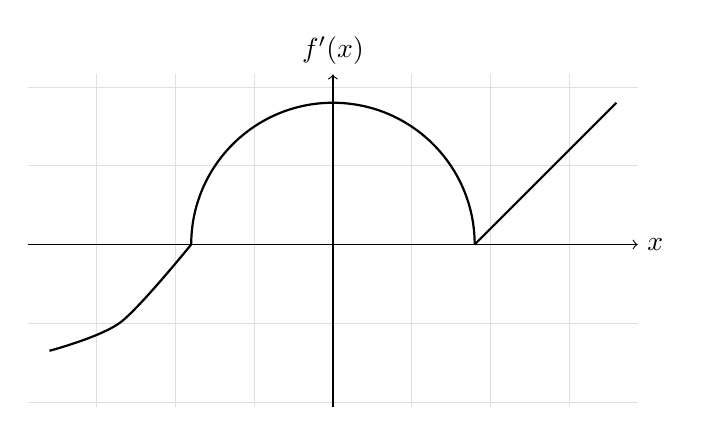
\begin{tikzpicture}[x=0.9cm,y=0.9cm]
  \draw[step=1cm,gray!25,very thin] (-4.3,-2.3) grid (4.3,2.4);
  \draw[->] (-4.3,0)--(4.3,0) node[right] {$x$};
  \draw[->] (0,-2.3)--(0,2.4) node[above] {$f'(x)$};
  \draw[thick] plot[smooth] coordinates {(-4,-1.5) (-3,-1.1) (-2,0)};
  \draw[thick] (-2,0) arc[start angle=180,end angle=0,radius=2];
  \draw[thick] (2,0)--(4,2);
\end{tikzpicture}
\end{center}
State the local extrema of $f$. \wsL
\end{probs}
\topicdivider{4.4}{Concavity and the Second Derivative Test}
\Needspace{10cm}
\begin{probs}
\prob{52.} Find the local extrema of $f$, using the second derivative test whenever applicable. Find the intervals of concavity, the $x$-coordinates of the inflection points, and sketch the graph.\[f(x)=\sqrt[5]{x}-1.\] \wsL
\end{probs}
\Needspace{10cm}
\begin{probs}
\prob{53.} Find the local extrema of $f$, using the second derivative test whenever applicable. Find the intervals of concavity, the $x$-coordinates of the inflection points, and sketch the graph.\[f(x)=\sqrt[3]{x^2}(3x+10).\] \wsL
\end{probs}
\Needspace{10cm}
\begin{probs}
\prob{54.} Sketch a continuous function $f$ satisfying all the conditions: \[\begin{gathered} f(0)=1,\quad f(2)=3,\quad f'(0)=f'(2)=0,\\ f'(x)<0\text{ if }|x-1|>1,\quad f'(x)>0\text{ if }|x-1|<1,\\ f''(x)>0\text{ if }x<1,\quad f''(x)<0\text{ if }x>1. \end{gathered}\] \wsL
\end{probs}
\Needspace{10cm}
\begin{probs}
\prob{55.} Sketch a continuous function $f$ satisfying all the conditions: \[\begin{gathered} f(0)=2,\quad f(2)=f(-2)=1,\quad f'(0)=0,\\ f'(x)>0\text{ if }x<0,\quad f'(x)<0\text{ if }x>0,\\ f''(x)<0\text{ if }|x|<2,\quad f''(x)>0\text{ if }|x|>2. \end{gathered}\] \wsL
\end{probs}
\Needspace{10cm}
\begin{probs}
\prob{56.} Sketch a continuous function $f$ satisfying all the conditions: \[f(1)=4,\qquad f'(x)>0\text{ if }x<1,\qquad f'(x)<0\text{ if }x>1,\qquad f''(x)>0\text{ for }x\ne1.\] \wsL
\end{probs}
\Needspace{10cm}
\begin{probs}
\prob{57.} Sketch a continuous function $f$ satisfying all the conditions. If $n$ is odd, $f(n)=1$ and $f'(n)=0$; if $n$ is even, $f(n)=0$ and $f'(n)$ does not exist. For every integer $n$, \[\begin{aligned} &f'(x)>0 &&\text{when }2n<x<2n+1,\\ &f'(x)<0 &&\text{when }2n-1<x<2n,\\ &f''(x)<0 &&\text{when }2n<x<2n+2. \end{aligned}\] \wsL
\end{probs}
\cfuheading
\Needspace{9cm}
\begin{probs}
\prob{} Use the table to decide whether each statement must be true.
\[
\begin{array}{c|cc}
x&f'(x)&f''(x)\\\hline
2&-2&0\\
3&0&0\\
4&0&3
\end{array}
\]
(a) $f$ must have a local maximum at $x=4$. (b) $f$ must have an inflection point at $x=2$. (c) $f$ must have an inflection point at $x=3$. \wsM
\end{probs}
\Needspace{8cm}
\begin{probs}
\prob{} Find all $x$-values where
\[
y=\frac1{20}x^5-\frac13x^4+\frac23x^3+70000
\]
has a point of inflection. Select from $-2,-1,0,1,2$. \wsM
\end{probs}
\Needspace{15cm}
\begin{probs}
\prob{} The graph below is $y=f'(x)$ for a differentiable function $f$ on $(-3,4)$. Find (a) the intervals where $f$ is concave up and (b) the $x$-values of all points of inflection.
\begin{center}
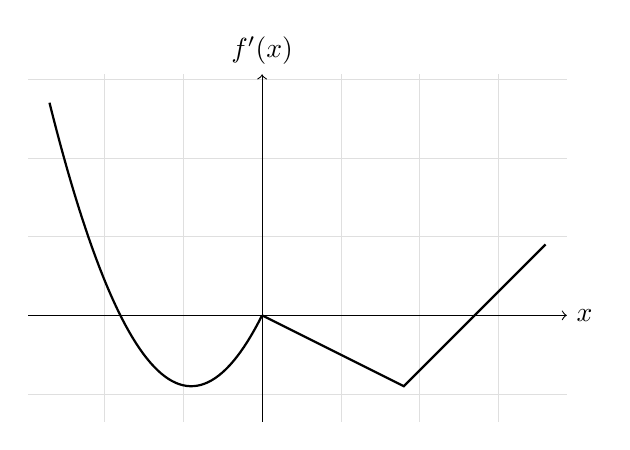
\begin{tikzpicture}[x=0.9cm,y=0.9cm]
  \draw[step=1cm,gray!25,very thin] (-3.3,-1.5) grid (4.3,3.4);
  \draw[->] (-3.3,0)--(4.3,0) node[right] {$x$};
  \draw[->] (0,-1.5)--(0,3.4) node[above] {$f'(x)$};
  \draw[thick,domain=-3:0,samples=60] plot (\x,{(\x+1)^2-1});
  \draw[thick] (0,0)--(2,-1)--(4,1);
\end{tikzpicture}
\end{center}
\wsM
\end{probs}
\clearpage
\begin{center}{\LARGE\bfseries Answer Key}\end{center}
\medskip
\noindent\textit{Answers correspond to questions 1--99.}
\begin{ans}
\ansitem{1} $\dfrac{1}{10}$.
\ansitem{2} (a) $-1$; (b) $1$; (c) DNE.
\ansitem{3} (C) $2$.
\ansitem{} $-\dfrac1{12}$.
\ansitem{} $7$.
\ansitem{} (a) $-2$; (b) $-1$; (c) DNE.
\ansitem{4} $\delta=\sqrt{16.1}-4\approx0.0124805$.
\ansitem{5} For any $\varepsilon>0$, choose $\delta=\varepsilon/5$. If $0<|x-2|<\delta$, then $|(5x-3)-7|=5|x-2|<5\delta=\varepsilon$.
\ansitem{6} (B) $\frac12$.
\ansitem{7} $-9$.
\ansitem{8} $0\le x^2f(x)\le cx^2$, and both bounding functions tend to $0$ as $x\to0$. The sandwich theorem gives $\lim_{x\to0}x^2f(x)=0$.
\ansitem{9} (D) $\cos x$.
\ansitem{} $4$.
\ansitem{} $-\dfrac1{10}$.
\ansitem{} (a) $0$; (b) DNE; (c) DNE.
\ansitem{10} (a) $-\infty$; (b) $\infty$; (c) DNE.
\ansitem{11} Vertical: $x=-5$. Horizontal: $y=1$.
\ansitem{12} (A) $0$.
\ansitem{} (C) $-\infty$.
\ansitem{} $-5$.
\ansitem{} Horizontal: $y=-1$. Vertical: $x=-5$ and $x=5$.
\ansitem{13} Removable discontinuity at $x=1$; $\lim_{x\to1}f(x)=-1\ne f(1)=2$.
\ansitem{14} $f$ is continuous on $[6,7]$, and $f(6)=69<100<138=f(7)$. By the intermediate value theorem, some $a\in(6,7)$ satisfies $f(a)=100$.
\ansitem{15} (C) $2$ only.
\ansitem{16} (a) $m=-4a$. (b) $y=-8x+11$.
\ansitem{17} (a) $48$, $16$, and $-16$ ft/sec, respectively. (b) $t=7$ sec. (c) $-112$ ft/sec.
\ansitem{18} (C) $\frac43$.
\ansitem{} (a) $4.1$; (b) $4$.
\ansitem{} (a) $v(t)=-32t$ ft/sec; (b) $v(2)=-64$ ft/sec.
\ansitem{} (B) $\dfrac16$.
\ansitem{19} (a) $f'(x)=3x^2-4$. (b) $(-\infty,\infty)$. (c) $y=8x-16$. (d) $\left(-\frac{2\sqrt3}{3},\frac{16\sqrt3}{9}\right)$ and $\left(\frac{2\sqrt3}{3},-\frac{16\sqrt3}{9}\right)$.
\ansitem{20} (a) No: $f'(0)$ does not exist as a finite number. (b) Yes: $f'(x)=1/(3x^{2/3})$ exists throughout the interval (with one-sided derivatives at its endpoints).
\ansitem{21} (C) $f'(2)=0$.
\ansitem{} $0$.
\ansitem{} (C) $4x^3$.
\ansitem{} $(-\infty,0)\cup(0,\infty)$.
\ansitem{22} $G'(v)=\dfrac{6v^2}{(v^3+1)^2}$.
\ansitem{23} $x=-5$ or $x=3$.
\ansitem{24} (E) $\dfrac{uv'w+u'vw-uvw'}{w^2}$.
\ansitem{} $\dfrac{13}{121}$.
\ansitem{} (D) $(x^2-4)(4x^3)+(x^4+2)(2x)$.
\ansitem{} (a) $-2$; (b) $-14$.
\ansitem{} $P=(2,4)$.
\ansitem{25} $h'(z)=\dfrac{2\sin z}{(1+\cos z)^2}$.
\ansitem{26} Tangent: $y-(1+\sqrt2)=-(2+\sqrt2)(x-\pi/4)$. Normal: $y-(1+\sqrt2)=\dfrac{x-\pi/4}{2+\sqrt2}$.
\ansitem{27} (E) $1-\frac\pi2$.
\ansitem{} $-\dfrac12$.
\ansitem{} $2$.
\ansitem{} $-4-2\sqrt3$.
\ansitem{28} (a) $\Delta y=\dfrac{1}{(x+\Delta x)^2}-\dfrac1{x^2}$ and $dy=-\dfrac{2}{x^3}\,dx$, where $dx=\Delta x$. (b) $\Delta y=-\dfrac7{363}$ and $dy=-\dfrac1{45}$.
\ansitem{29} The pressure difference increases by approximately $40\%$.
\ansitem{30} (D) $2.7$.
\ansitem{31} $f'(x)=\dfrac{\cos\sqrt{x}}{2\sqrt{x}}+\dfrac{\cos x}{2\sqrt{\sin x}}$ (where the terms are defined).
\ansitem{32} $p(3)=-2$ and $p'(3)=24$.
\ansitem{33} (D) $12$.
\ansitem{} (B) $3\tan(2)\sec^2(2)$.
\ansitem{} $f(1.1)\approx2.3$.
\ansitem{} $144$.
\ansitem{34} $y'=\dfrac{1-y\cos(xy)}{x\cos(xy)}$.
\ansitem{35} $y''=-\dfrac{3}{4y^3}$ for $y\ne0$.
\ansitem{36} (D) $\frac34$.
\ansitem{} $1$.
\ansitem{} (D) $-\pi$.
\ansitem{} $(1,-\sqrt2)$ and $(-1,\sqrt2)$.
\ansitem{37} The volume is increasing at $\dfrac{21\pi}{160}$ cm$^3$/min.
\ansitem{38} $\dfrac{d\theta}{dt}=-\dfrac16$ rad/sec; the angle is decreasing.
\ansitem{39} (D) $\frac43$ m/s.
\ansitem{} (a) $\dfrac32$ ft/sec; (b) $\dfrac92$ ft/sec; (c) $-\dfrac1{16}$ rad/sec.
\ansitem{} (a) $2\sqrt2$ cm/sec; (b) $24$ cm$^2$/sec.
\ansitem{40} (a) $2$; (b) $-7$; (c) $-14$; (d) $21$; (e) $-\dfrac{10}{9}$; (f) $-\dfrac{19}{27}$.
\ansitem{41} Yes. Both pieces have value $27$ at $x=2$, and both one-sided derivatives equal $54$, so $f'(2)=54$.
\ansitem{42} (A) $f''(g(x))[g'(x)]^2+f'(g(x))g''(x)$.
\ansitem{43} Absolute maximum $20$ at $x=-1$; absolute minimum $-\frac43$ at $x=\frac53$.
\ansitem{44} $r=-1,-\frac1{\sqrt5},\frac1{\sqrt5},1$.
\ansitem{45} (E) $9$.
\ansitem{} (a) $3$; (b) four critical numbers, at $x=-2,-1,0,1$; (c) local maxima at $x=-2$ and $x=1$.
\ansitem{} (D) $20$.
\ansitem{} $y=x^2$ is increasing on $(0,\infty)$; $y=x^3$ is increasing on $(-\infty,\infty)$.
\ansitem{} $0$ and $8$.
\ansitem{46} The polynomial is continuous and differentiable, and $f(-3)=f(3)=118$. The only number is $c=0$.
\ansitem{47} Yes. The average slope is $2$, and $c=\frac{2-\sqrt7}{3}$ is the only solution in $(-1,1)$.
\ansitem{48} (B) intersect no more than once.
\ansitem{} Select (ii) continuous on $[2,5]$ and (iii) differentiable on $(2,5)$.
\ansitem{} (A)$\to$(1), (B)$\to$(2), (C)$\to$(3), (D)$\to$(4).
\ansitem{} $c=2$.
\ansitem{49} Increasing on $(-\infty,\frac35]$ and $[1,\infty)$; decreasing on $[\frac35,1]$. Local maximum $f(\frac35)=\frac{216}{625}$; local minimum $f(1)=0$. The critical number $x=0$ is not an extremum.
\ansitem{50} Decreasing on $[0,\frac\pi3]$ and $[\frac{5\pi}3,2\pi]$; increasing on $[\frac\pi3,\frac{5\pi}3]$. Local minimum $f(\frac\pi3)=\frac\pi6-\frac{\sqrt3}{2}$; local maximum $f(\frac{5\pi}3)=\frac{5\pi}6+\frac{\sqrt3}{2}$.
\ansitem{51} One valid answer is $f(x)=\frac74(|x|-2)^2-4$. It has local minima at $(-2,-4)$ and $(2,-4)$ and a cusp-shaped local maximum at $(0,3)$.
\ansitem{} Select: local maximum at $x=1$; increasing on $(-\infty,0)\cup(0,1)$; decreasing on $(1,\infty)$.
\ansitem{} Local minimum at $x=-2$ and no local maximum.
\ansitem{52} No local extrema; increasing on $(-\infty,\infty)$. Concave up on $(-\infty,0)$ and down on $(0,\infty)$. Inflection point $(0,-1)$, with a vertical tangent.
\ansitem{53} Local maximum $f(-\frac43)=4\sqrt[3]{6}$; local minimum $f(0)=0$. Concave down on $(-\infty,0)$ and $(0,\frac23)$; concave up on $(\frac23,\infty)$. Inflection point $\left(\frac23,4\sqrt[3]{12}\right)$; cusp at the origin.
\ansitem{54} Decreasing on $(-\infty,0)$, increasing on $(0,2)$, and decreasing on $(2,\infty)$. Local minimum $(0,1)$; local maximum $(2,3)$. Concave up for $x<1$, concave down for $x>1$; inflection at $x=1$ (height not determined).
\ansitem{55} Increasing on $(-\infty,0)$ and decreasing on $(0,\infty)$, with local maximum $(0,2)$. Concave up on $(-\infty,-2)$ and $(2,\infty)$; concave down on $(-2,2)$. Inflection points $(-2,1)$ and $(2,1)$.
\ansitem{56} Increasing on $(-\infty,1)$ and decreasing on $(1,\infty)$, with local maximum $(1,4)$. Concave up on both sides of $x=1$. One valid shape has a cusp at $(1,4)$, for example $f(x)=4-\sqrt{|x-1|}$.
\ansitem{57} One valid graph is $f(x)=\left|\sin\frac{\pi x}{2}\right|$: concave-down arches rise from each even-integer corner $(2n,0)$ to a horizontal maximum $(2n+1,1)$ and return to $(2n+2,0)$.
\ansitem{} (a) False; (b) False; (c) False.
\ansitem{} $x=0$ only.
\ansitem{} (a) Concave up on $(-1,0)\cup(2,4)$; (b) inflection points at $x=-1,0,2$.
\end{ans}
\clearpage
% === SOURCELIST ===
\iffalse
\begin{center}{\LARGE\bfseries Where These Questions Came From}\end{center}
\medskip
\noindent This guide covers textbook Sections 2.1 through 4.4. For 2.1--4.2, each group uses two textbook exercises not listed anywhere in the 2026--27 calendar's Solve, Recommended Continued Practice, Opener, Challenge, or IP columns, plus one question from the supplied AP packet. The final nine questions reproduce every 4.3--4.4 textbook exercise already collected in the 4.3--4.6 study guide.
\medskip
\begin{multicols}{2}
\noindent\textbf{Section 2.1}
\begin{itemize}[leftmargin=1.5em,itemsep=1pt,topsep=2pt]
\item[] \textbf{1} $=$ 2.1 \#18
\item[] \textbf{2} $=$ 2.1 \#26
\item[] \textbf{3} $=$ AP Packet p. 13, BC 2 (1993)
\end{itemize}
\smallskip
\noindent\textbf{Section 2.2}
\begin{itemize}[leftmargin=1.5em,itemsep=1pt,topsep=2pt]
\item[] \textbf{4} $=$ 2.2 \#9
\item[] \textbf{5} $=$ 2.2 \#16
\item[] \textbf{6} $=$ AP Packet p. 4, BC 6 (1969)
\end{itemize}
\smallskip
\noindent\textbf{Section 2.3}
\begin{itemize}[leftmargin=1.5em,itemsep=1pt,topsep=2pt]
\item[] \textbf{7} $=$ 2.3 \#28
\item[] \textbf{8} $=$ 2.3 \#65
\item[] \textbf{9} $=$ AP Packet p. 5, BC 10 (1988)
\end{itemize}
\smallskip
\noindent\textbf{Section 2.4}
\begin{itemize}[leftmargin=1.5em,itemsep=1pt,topsep=2pt]
\item[] \textbf{10} $=$ 2.4 \#3
\item[] \textbf{11} $=$ 2.4 \#34
\item[] \textbf{12} $=$ AP Packet p. 2, BC 35 (1988)
\end{itemize}
\smallskip
\noindent\textbf{Section 2.5}
\begin{itemize}[leftmargin=1.5em,itemsep=1pt,topsep=2pt]
\item[] \textbf{13} $=$ 2.5 \#16
\item[] \textbf{14} $=$ 2.5 \#59
\item[] \textbf{15} $=$ AP Packet p. 2, BC 5 (1988)
\end{itemize}
\smallskip
\noindent\textbf{Section 3.1}
\begin{itemize}[leftmargin=1.5em,itemsep=1pt,topsep=2pt]
\item[] \textbf{16} $=$ 3.1 \#2
\item[] \textbf{17} $=$ 3.1 \#16
\item[] \textbf{18} $=$ AP Packet p. 3, BC 4 (1973)
\end{itemize}
\smallskip
\noindent\textbf{Section 3.2}
\begin{itemize}[leftmargin=1.5em,itemsep=1pt,topsep=2pt]
\item[] \textbf{19} $=$ 3.2 \#4
\item[] \textbf{20} $=$ 3.2 \#22
\item[] \textbf{21} $=$ AP Packet p. 3, BC 8 (1985)
\end{itemize}
\smallskip
\noindent\textbf{Section 3.3}
\begin{itemize}[leftmargin=1.5em,itemsep=1pt,topsep=2pt]
\item[] \textbf{22} $=$ 3.3 \#19
\item[] \textbf{23} $=$ 3.3 \#45
\item[] \textbf{24} $=$ AP Packet p. 4, BC 4 (1988)
\end{itemize}
\smallskip
\noindent\textbf{Section 3.4}
\begin{itemize}[leftmargin=1.5em,itemsep=1pt,topsep=2pt]
\item[] \textbf{25} $=$ 3.4 \#13
\item[] \textbf{26} $=$ 3.4 \#30
\item[] \textbf{27} $=$ AP Packet p. 5, BC 6 (1985)
\end{itemize}
\smallskip
\noindent\textbf{Section 3.5}
\begin{itemize}[leftmargin=1.5em,itemsep=1pt,topsep=2pt]
\item[] \textbf{28} $=$ 3.5 \#3
\item[] \textbf{29} $=$ 3.5 \#41
\item[] \textbf{30} $=$ AP Packet p. 4, BC 92 (1998)
\end{itemize}
\smallskip
\noindent\textbf{Section 3.6}
\begin{itemize}[leftmargin=1.5em,itemsep=1pt,topsep=2pt]
\item[] \textbf{31} $=$ 3.6 \#53
\item[] \textbf{32} $=$ 3.6 \#82
\item[] \textbf{33} $=$ AP Packet p. 7, BC 39 (1973)
\end{itemize}
\smallskip
\noindent\textbf{Section 3.7}
\begin{itemize}[leftmargin=1.5em,itemsep=1pt,topsep=2pt]
\item[] \textbf{34} $=$ 3.7 \#12
\item[] \textbf{35} $=$ 3.7 \#29
\item[] \textbf{36} $=$ AP Packet p. 8, BC 3 (1998)
\end{itemize}
\smallskip
\noindent\textbf{Section 3.8}
\begin{itemize}[leftmargin=1.5em,itemsep=1pt,topsep=2pt]
\item[] \textbf{37} $=$ 3.8 \#34
\item[] \textbf{38} $=$ 3.8 \#42
\item[] \textbf{39} $=$ AP Packet p. 9, BC 37 (1988)
\end{itemize}
\smallskip
\noindent\textbf{Section 3.9}
\begin{itemize}[leftmargin=1.5em,itemsep=1pt,topsep=2pt]
\item[] \textbf{40} $=$ 3.9 \#63
\item[] \textbf{41} $=$ 3.9 \#66
\item[] \textbf{42} $=$ AP Packet p. 7, BC 5 (1998)
\end{itemize}
\smallskip
\noindent\textbf{Section 4.1}
\begin{itemize}[leftmargin=1.5em,itemsep=1pt,topsep=2pt]
\item[] \textbf{43} $=$ 4.1 \#8
\item[] \textbf{44} $=$ 4.1 \#16
\item[] \textbf{45} $=$ AP Packet p. 13, BC 27 (1973)
\end{itemize}
\smallskip
\noindent\textbf{Section 4.2}
\begin{itemize}[leftmargin=1.5em,itemsep=1pt,topsep=2pt]
\item[] \textbf{46} $=$ 4.2 \#5
\item[] \textbf{47} $=$ 4.2 \#17
\item[] \textbf{48} $=$ AP Packet p. 3, BC 15 (1969)
\end{itemize}
\smallskip
\noindent\textbf{Section 4.3}
\begin{itemize}[leftmargin=1.5em,itemsep=1pt,topsep=2pt]
\item[] \textbf{49} $=$ 4.3 \#7
\item[] \textbf{50} $=$ 4.3 \#19
\item[] \textbf{51} $=$ 4.3 \#35
\end{itemize}
\smallskip
\noindent\textbf{Section 4.4}
\begin{itemize}[leftmargin=1.5em,itemsep=1pt,topsep=2pt]
\item[] \textbf{52} $=$ 4.4 \#9
\item[] \textbf{53} $=$ 4.4 \#11
\item[] \textbf{54} $=$ 4.4 \#31
\item[] \textbf{55} $=$ 4.4 \#33
\item[] \textbf{56} $=$ 4.4 \#34
\item[] \textbf{57} $=$ 4.4 \#37
\end{itemize}
\smallskip
\end{multicols}
\fi
\begin{center}{\LARGE\bfseries Where These Questions Came From}\end{center}
\medskip
\noindent This guide contains 99 questions. Within each section, the original textbook and AP-packet questions come first, followed by every supplied Section Quiz screenshot for that section. The sources below are listed in the same order as the question numbers in each range.
\medskip
\begin{multicols}{2}
\small
\noindent\textbf{Section 2.1 (Questions 1--6)}\\
2.1 \#18; 2.1 \#26; AP Packet p. 13, BC 2 (1993); Section Quiz pp. 2--4.

\smallskip
\noindent\textbf{Section 2.2 (Questions 7--9)}\\
2.2 \#9; 2.2 \#16; AP Packet p. 4, BC 6 (1969).

\smallskip
\noindent\textbf{Section 2.3 (Questions 10--15)}\\
2.3 \#28; 2.3 \#65; AP Packet p. 5, BC 10 (1988); Section Quiz pp. 2--4.

\smallskip
\noindent\textbf{Section 2.4 (Questions 16--21)}\\
2.4 \#3; 2.4 \#34; AP Packet p. 2, BC 35 (1988); Section Quiz pp. 2--4.

\smallskip
\noindent\textbf{Section 2.5 (Questions 22--24)}\\
2.5 \#16; 2.5 \#59; AP Packet p. 2, BC 5 (1988).

\smallskip
\noindent\textbf{Section 3.1 (Questions 25--30)}\\
3.1 \#2; 3.1 \#16; AP Packet p. 3, BC 4 (1973); Section Quiz pp. 2--4.

\smallskip
\noindent\textbf{Section 3.2 (Questions 31--36)}\\
3.2 \#4; 3.2 \#22; AP Packet p. 3, BC 8 (1985); Section Quiz pp. 2--4.

\smallskip
\noindent\textbf{Section 3.3 (Questions 37--43)}\\
3.3 \#19; 3.3 \#45; AP Packet p. 4, BC 4 (1988); Section Quiz pp. 2--5.

\smallskip
\noindent\textbf{Section 3.4 (Questions 44--49)}\\
3.4 \#13; 3.4 \#30; AP Packet p. 5, BC 6 (1985); Section Quiz pp. 2--4.

\smallskip
\noindent\textbf{Section 3.5 (Questions 50--52)}\\
3.5 \#3; 3.5 \#41; AP Packet p. 4, BC 92 (1998).

\smallskip
\noindent\textbf{Section 3.6 (Questions 53--58)}\\
3.6 \#53; 3.6 \#82; AP Packet p. 7, BC 39 (1973); Section Quiz pp. 2--4.

\smallskip
\noindent\textbf{Section 3.7 (Questions 59--64)}\\
3.7 \#12; 3.7 \#29; AP Packet p. 8, BC 3 (1998); Section Quiz pp. 2--4.

\smallskip
\noindent\textbf{Section 3.8 (Questions 65--69)}\\
3.8 \#34; 3.8 \#42; AP Packet p. 9, BC 37 (1988); Section Quiz pp. 2--3.

\smallskip
\noindent\textbf{Section 3.9 (Questions 70--72)}\\
3.9 \#63; 3.9 \#66; AP Packet p. 7, BC 5 (1998).

\smallskip
\noindent\textbf{Section 4.1 (Questions 73--79)}\\
4.1 \#8; 4.1 \#16; AP Packet p. 13, BC 27 (1973); Section Quiz pp. 2--5.

\smallskip
\noindent\textbf{Section 4.2 (Questions 80--85)}\\
4.2 \#5; 4.2 \#17; AP Packet p. 3, BC 15 (1969); Section Quiz pp. 2--4.

\smallskip
\noindent\textbf{Section 4.3 (Questions 86--90)}\\
4.3 \#7; 4.3 \#19; 4.3 \#35; Section Quiz pp. 1--2.

\smallskip
\noindent\textbf{Section 4.4 (Questions 91--99)}\\
4.4 \#9; 4.4 \#11; 4.4 \#31; 4.4 \#33; 4.4 \#34; 4.4 \#37; Section Quiz pp. 2--4.
\end{multicols}
\end{document}
